\begin{figure}[htbp]
\centering
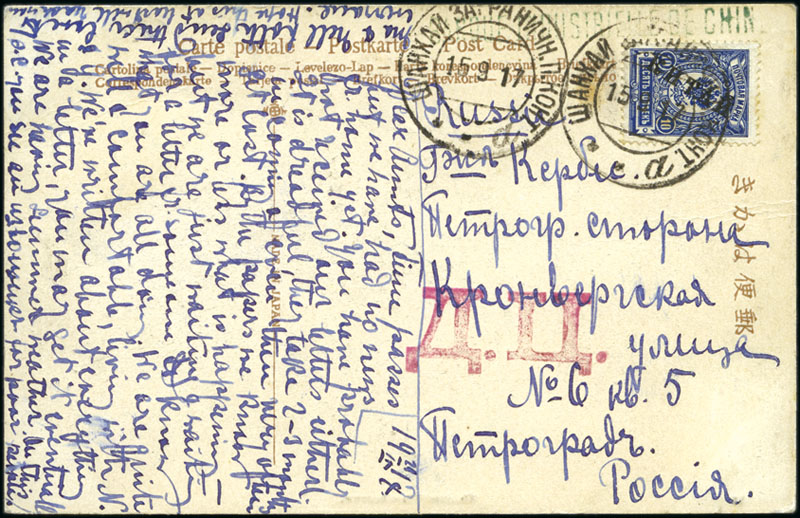
\includegraphics[width=.95\textwidth]{../russian-post-offices-in-china/10086.jpg}
\caption{
10086	SHANGHAI: 1917 Japanese postcard to Petrograd with "KITAI" 10k tied
by Shanghai 15.9.17 cds (T\&S type 8A), with magenta censor hs adjacent, 
the sender complaining that letters take 2-3 months in coming and often 
get lost, fine.
Note: Origin of the illustration in "Russische Postcensuur 1914-1918" 
p.86 by A. Speeckaert.
\euro 300.00 
}  
\end{figure}

\begin{figure}[htbp]
\centering
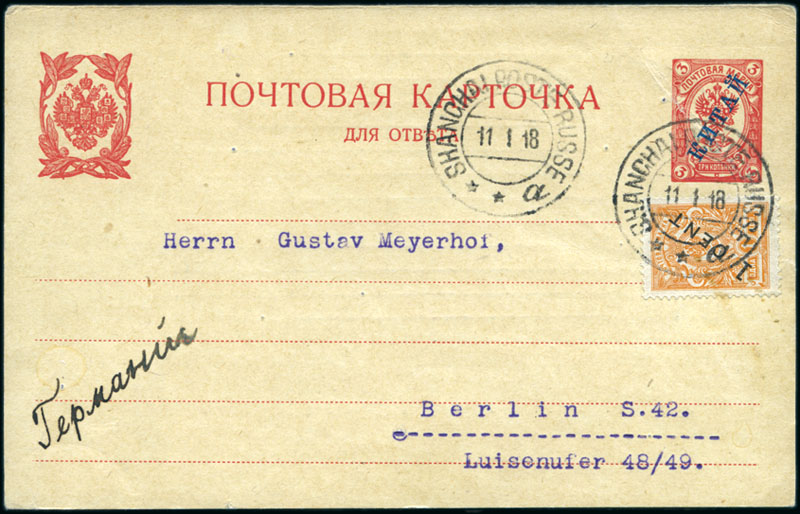
\includegraphics[width=.95\textwidth]{../russian-post-offices-in-china/10087.jpg}
\caption{
10087SHANGHAI: 1917 3k "KITAI" postal stationery card, used in combination 
with 1 CENT on 1k, tied by Shanghai Post Russe 11.1.18 cds (T\&S type 6A), 
very fine \& scarce

Note: Owing to wartime depreciation of the rouble, in 1917 Russian stamps 
for use in China proper were surcharged (and payment required) in Chinese 
currency. This item shows, however, that stamps and stationery 
denominated in Russian currency were still accepted after 1917 
when supplied by the customer
\euro 200.00  
}  
\end{figure}


\begin{figure}[htbp]
\centering
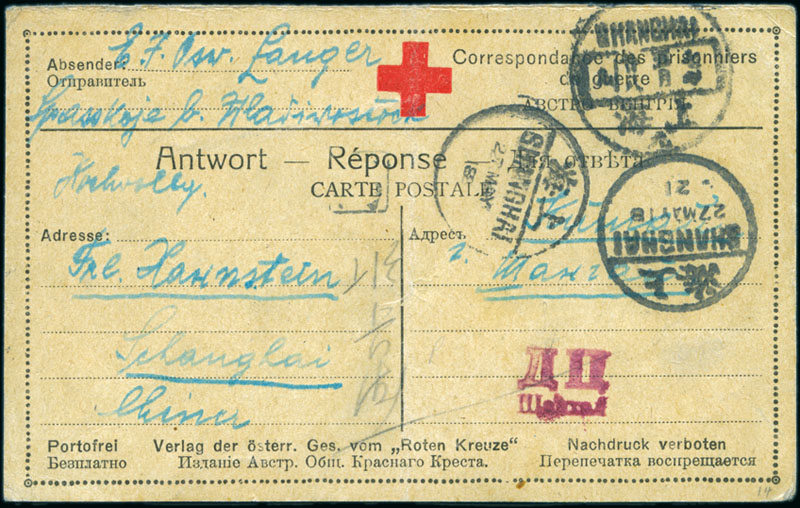
\includegraphics[width=.95\textwidth]{../russian-post-offices-in-china/10088.jpg}
\caption{
10088SHANGHAI: 1918 Red Cross post-free card from a P.O.W. at Spasskoe (Siberia) 
to Shanghai, received by the Chinese P.O. and passed to the Russian P.O. 
where a magenta two-line censor hs was applied (Speeckaert type 6, given 
highest rarity rating 5), fine.
NOTE: Origin of the illustration in "Russische Postcensuur 1914-1918" 
p.86 by A. Speeckaert.
\euro 400.00 
}  
\end{figure}


\begin{figure}[htbp]
\centering
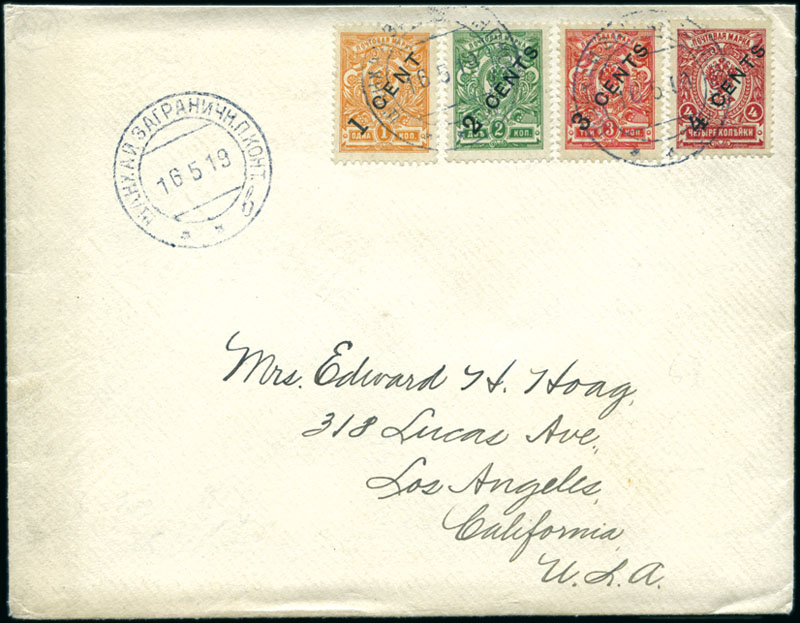
\includegraphics[width=.95\textwidth]{../russian-post-offices-in-china/10089.jpg}
\caption{
10089SHANGHAI: 1919 Cover to the USA with Russia Chinese surcharged 1c on 1k, 
2c on 2k, 3c on 3k and 4c on 4k paying the foreign letter rate, tied by 
Shanghai 16.5.19 cds (T\&S type 8C), a very fine and neat cover.

NOTE: From the beginning the Russian P.O.s in China had accepted payment 
in Chinese currency at a rate of 1c for 1k. Russian money was also accepted. 
However, after the Revolution of 1917 there followed a heavy depreciation in 
the Rouble which led the Postal Administration to insist on payment in 
Chinese currency only, hence the surcharged set of stamps in Chinese 
cents and dollars.
\euro 300.00  
}  
\end{figure}

\begin{figure}[htbp]
\centering
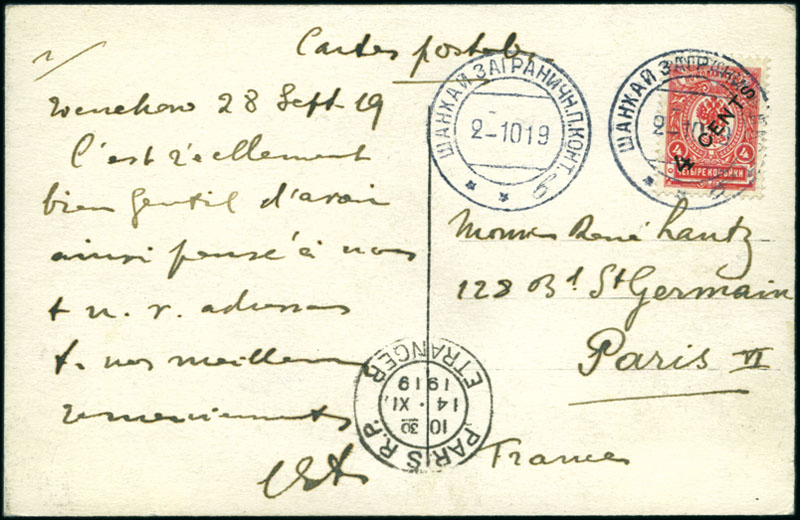
\includegraphics[width=.95\textwidth]{../russian-post-offices-in-china/10090.jpg}
\caption{
10090	SHANGHAI: 1919 Postcard to France with Russia Chinese surcharged 4c on 4k
tied by 2.10.19 cds (T\&S type 8C), Paris arrival, very fine
\euro 200.00  
}  
\end{figure}

\begin{figure}[htbp]
\centering
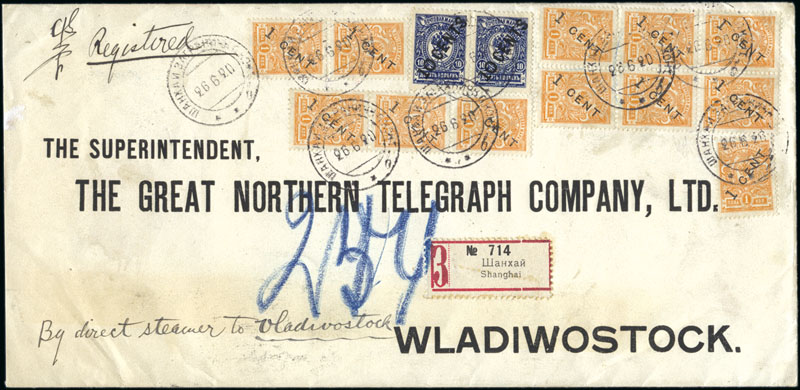
\includegraphics[width=.95\textwidth]{../russian-post-offices-in-china/10091.jpg}
\caption{
10091		ZoomSHANGHAI: 1920 Large envelope registered to Vladivostok
with Russia Chinese surcharged 1c on 1k (12) and 10c on 10k (2), all
tied by Shanghai 26.6.20 cds (T\&S type 8C), with reg'd label in 
Cyrillic and English adjacent, Vladivostok bs, a fine and attractive 
multple franking, and a late usage (the Russian P.O.s in China were closed November 1920)
\euro 400.00 
}  
\end{figure}  